\section{Artificial Neural Network} 
In this section, we will describe and reflect upon the result of the \gls{ann} experiments conducted in this project. We will also evaluate the performance of the \gls{ann} architecture proposed by \cite{} as we mentioned in \textbf{\autoref{}}. For the evaluation of the 
 
\subsection{Initial Model}
Initially, we have tested a variety of models, and we end up with the following initial model, which comparatively speaking performs well.
For our initial model, we have tested a model with the following specification:

\begin{table}[H]
    \centering
    \caption{Model Specification for initial \gls{ann} experiment.}
    \begin{tabular}{m{0.3\textwidth}m{0.2\textwidth} m{0.2\textwidth}}
        \hline
        \multicolumn{1}{c}{\textbf{Description}} & \multicolumn{1}{c}{\textbf{Neurons}} & \multicolumn{1}{c}{\textbf{Activation}}\\
        \hline
        
        Input Layer         &   \multicolumn{1}{c}{$N$} & \multicolumn{1}{c}{None}        \\
        1. Hidden Layer     &   \multicolumn{1}{c}{$\frac{1}{4}N$}  & \multicolumn{1}{c}{ReLU}     \\
        2. Hidden Layer     &   \multicolumn{1}{c}{$\frac{1}{2}N$}  & \multicolumn{1}{c}{ReLU}     \\
        Output Layer     &   \multicolumn{1}{c}{$1$}  & \multicolumn{1}{c}{None}     \\
        \hline
    \end{tabular}
    \label{tab:NN01}
\end{table}

% \begin{itemize}
%     \item A hidden layer with neurons amounting to half of the input neurons and relu activation function
%     \item A hidden layer with neurons amounting to $1/4$ of the input neurons and relu activation function
%     \item A hidden layer with neurons amounting to half of the input neurons and relu activation function
%     \item A output layer with one neuron
%     \item As gradient descent, Adam has been used with a learning rate of 0.01 in a batch size of 32.
% \end{itemize}
Models with the specification mentioned in \textbf{\autoref{tab:NN01}} have been trained for each site and for each X, Y, and floor. We have decided to implement models for X, Y, and floor separately as we believe that a more specific model will have better performance as it does not need to focus on more than one prediction. The models have been trained with the optimiser Adam, which is a variation of stochastic gradient descent, and in batches of size 32. The models have been trained for 100 epochs, but with early stopping with patience of 10 epoch in the validation loss. This means that if the validation loss does not improve in 10 epochs, the training of the model will end.

\subsubsection{Results of First Test}
The results of this model specification varies depending on the whether the prediction is X,Y or floor. We will evaluate each of them respectively. For the Y-values, when looking at the development of the training and validation loss, we can see that for most of the cases the initial loss is high. This can be seen on (a) on \textbf{\autoref{fig:NN01}}. Even when investigating the training after the initial training period, we can still see that the model struggles to find the optimal state and the final loss furthermore also seems to be quite high. This is indicated on (b) on \textbf{\autoref{fig:NN01}}. Furthermore, the mean of the \gls{mse}s for all sites for the training data and validation data are at 9372 and 2407.32, respectively. This further illustrates the issue of not finding an optima. 

\begin{figure}[H]
\centering
  \SetFigLayout{1}{2}
  \subfigure[]{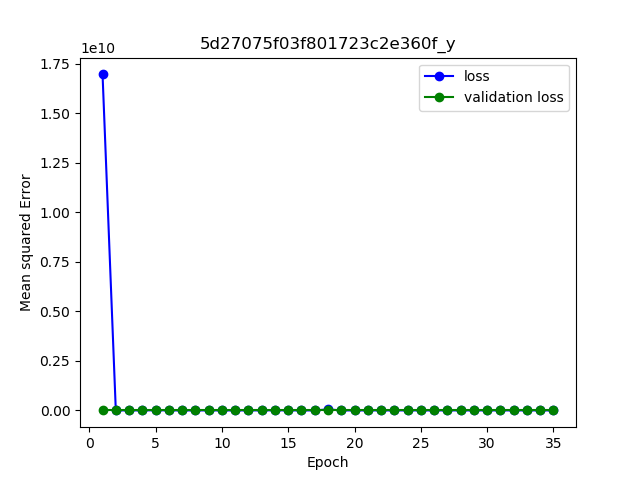
\includegraphics{Images/Experiments/NN/1.initial/all/5d27075f03f801723c2e360f_y.png}
  }
  \hfill
  \subfigure[]{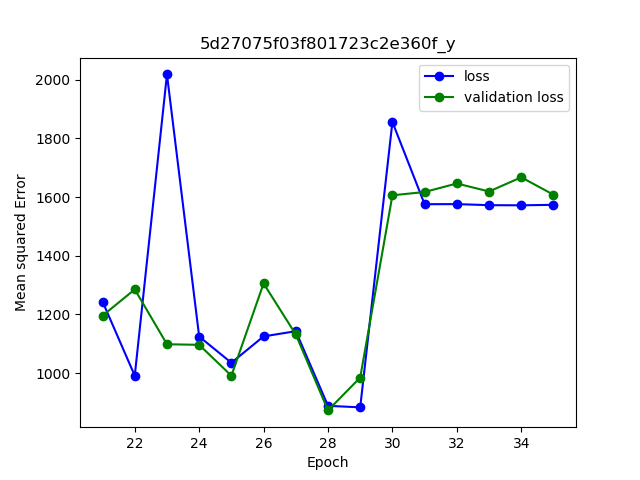
\includegraphics{Images/Experiments/NN/1.initial/after20/5d27075f03f801723c2e360f_y.png}}
  \caption{The performance for a site.}
  \label{fig:NN01}
\end{figure}
% \begin{figure}[h]
%     \centering
%     \includegraphics[scale=0.5]{Images/Experiments/NN/expr01/5da138764db8ce0c98bcaa46_y(0).png}
%     \caption{Training with all epochs}
%     \label{fig:NN_01}
% \end{figure}
% \begin{figure}[h]
%     \centering
%     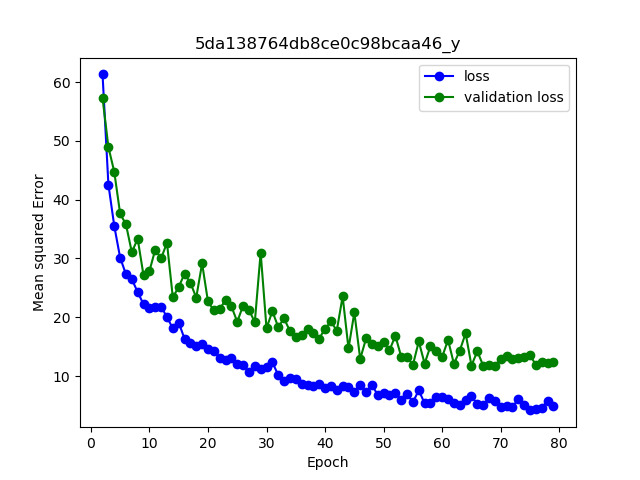
\includegraphics[scale=0.5]{Images/Experiments/NN/expr01/5da138764db8ce0c98bcaa46_y.png}
%     \caption{Training with epoch 2 and onward}
%     \label{fig:NN_02}
% \end{figure}
As with Y, we notice the same tendencies with results for the X predictions. The result of the same site as in \textbf{\autoref{fig:NN01}} is shown for the result for X estimations in \textbf{\autoref{fig:NN01_x}}. The mean of the \gls{mse}s for the sites for the X estimations are at 4967 and 3077 for the training and validation datasets, respectively.
\begin{figure}[H]
    \centering
    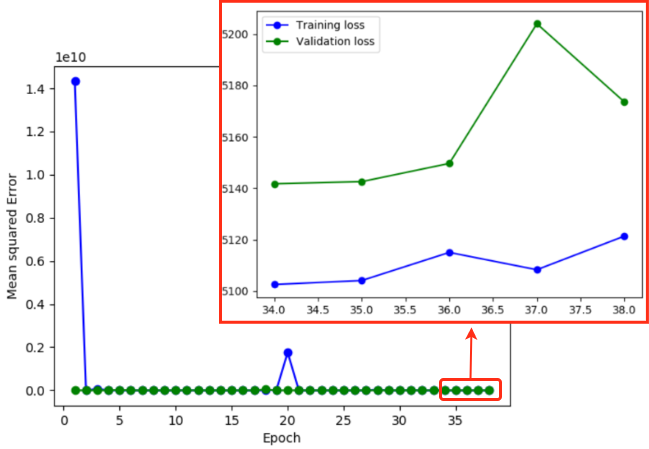
\includegraphics[scale=0.4]{Images/Experiments/NN/1.initial/5d27075f03f801723c2e360f_x.png}
    \caption{Results for site 5d27075f03f801723c2e360f for X estimations.}
    \label{fig:NN01_x}
\end{figure}
Among the estimations, we observe the worst behaviour for the floor estimations, when considering the mean of \gls{mse}s, which are at $166586.22$ and $8538.34$ for the training and validation data, respectively. However, for most of the sites for the floor predictions, we achieve good results, but the overall mean is dragged up due to a few extreme results. One of the good results is displayed in \textbf{\autoref{fig:NN01_floor}}.
\begin{figure}[H]
    \centering
    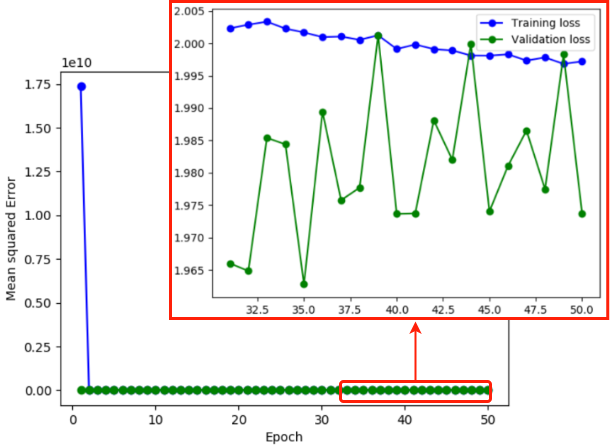
\includegraphics[scale=0.4]{Images/Experiments/NN/1.initial/5d27075f03f801723c2e360f_floor.png}
    \caption{Results for site 5d27075f03f801723c2e360f for floor estimations.}
    \label{fig:NN01_floor}
\end{figure}

The overall issue with struggling to find the optima, which we observe especially for the X and Y estimations, can have a number of reasons. The reasoning for this, which we think is most likely, might be due to a high learning rate or due to the model being unable to properly localise the optimum in the raw dataset. To this end, we will try to decrease the learning rate in one experiment and try training with the normalised dataset in another experiment.


\subsubsection{Results of Second Test}
After conducting the experiment with an adjusted learning rate of 0.001, we achieve better results compared to the initial experiment for all the models. This is deemed from the mean of \gls{mse}s on both training and validation dataset. 

%The results for the site, which we have shown for the earlier experiment, is shown here. 
%In the initial experiment, we end up with a loss around 1600, while in with the adjusted learning rate we achieve a loss around 50. This is further illustrated by the mean of the \gls{mse}s on the training and validation dataset, which is 1590 and 2191 for the initial experiment, while it becomes 516 and 475 for the second experiment for the training and validation \gls{mse}s, respectively.
% \begin{figure}[H]
% \centering
%   \SetFigLayout{1}{2}
%   \subfigure[]{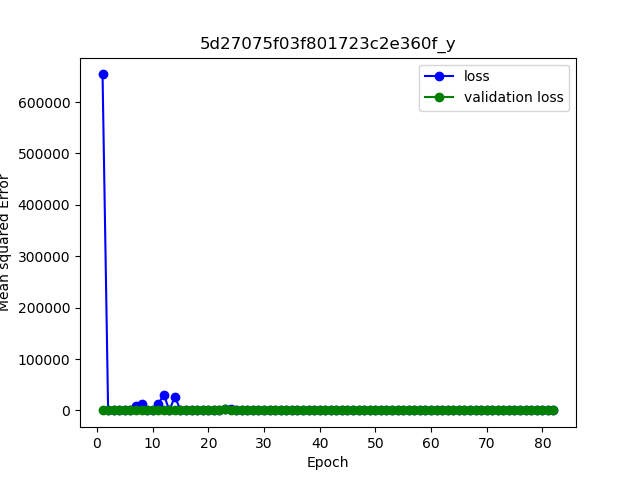
\includegraphics{Images/Experiments/NN/2.adjustedLR/5d27075f03f801723c2e360f_y_all.png}
%   }
%   \hfill
%   \subfigure[]{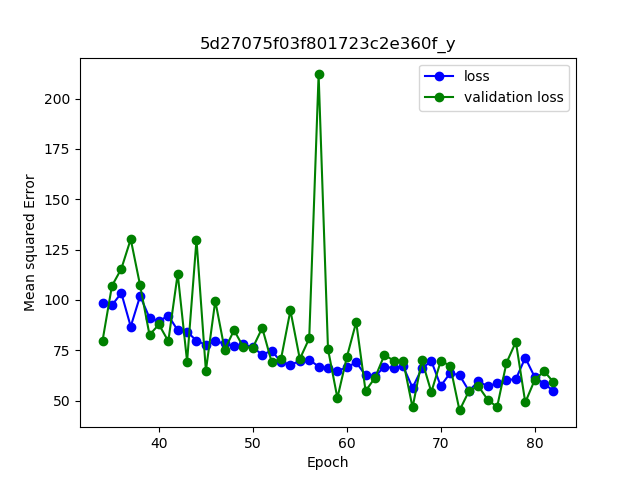
\includegraphics{Images/Experiments/NN/2.adjustedLR/5d27075f03f801723c2e360f_y_34.png}
%   }
%   \caption{The performance for a site.}
%   \label{fig:NN02}
% \end{figure}
\begin{figure}[H]
\centering
  \SetFigLayout{1}{2}
  \subfigure[]{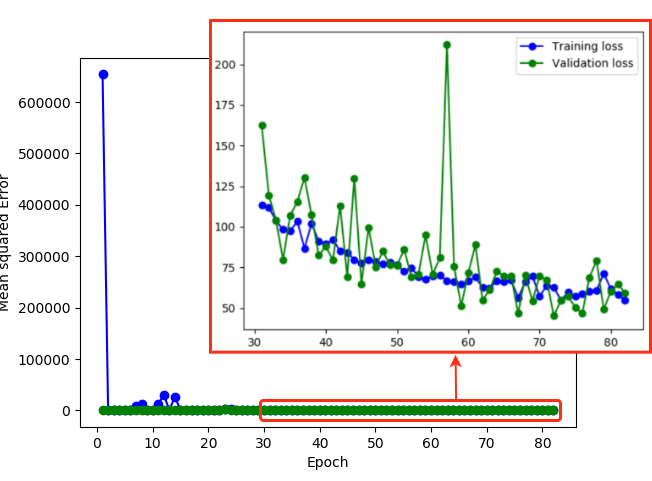
\includegraphics{Images/Experiments/NN/1.initial/exp2_y_5d27075f03f801723c2e360f.png}
  }
  \hfill
  \subfigure[]{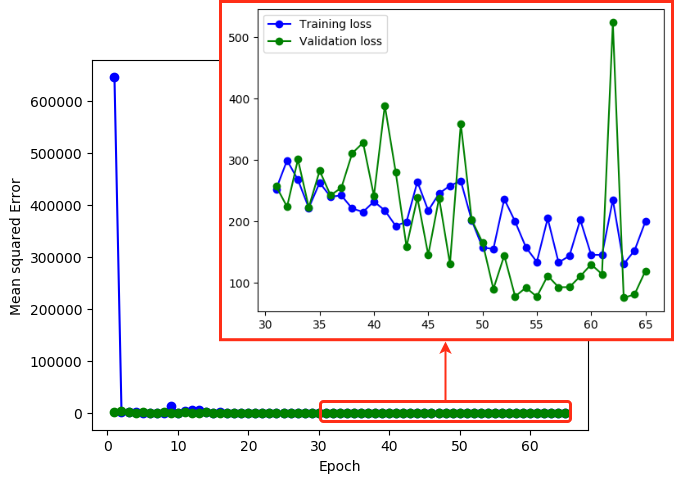
\includegraphics{Images/Experiments/NN/1.initial/exp2_x_5d27075f03f801723c2e360f.png}}
  \caption{Results for site 5d27075f03f801723c2e360f for y estimations (a) and x estimations (b).}
  \label{fig:exp2}
\end{figure}

\textbf{\autoref{fig:exp2}} displays the result of the X and Y estimations. For the X estimations, the mean of \gls{mse}s are 669 \& 2298.73 for training and validation, respectively. This is still a quite huge gap between the training and validation loss. For the Y estimations, we achieve a mean of \gls{mse}s of 1159 for training and 230.59 for validation.  Lastly for the Floor model, we achieve 8891 for training dataset and 533.03 for validation dataset. We see an improvement in comparison to the initial test, but overall the performance still does not seem ideal.

%\begin{figure}[H]
   % \centering
   % \includegraphics[scale=0.5]{Images/Experiments/NN/1.initial/e%xp2_floor_5d27075f03f801723c2e360f.png}
   % \caption{Results for site 5d27075f03f801723c2e360f for floor %estimations.}
   % \label{fig:exp2_floor}
%\end{figure}

\subsubsection{Results of Third Test}
We have also conducted the experiment with a normalised dataset. The data is normalised through Min-Max Normalisation, which is used to scale features as mentioned in \autoref{sec:minmaxnormalisation}. Applying this to the \gls{ann} model should lead to a decrease in the loss and an increase in the performance of the model.

\begin{figure}[H]
\centering
  \SetFigLayout{1}{2}
  \subfigure[]{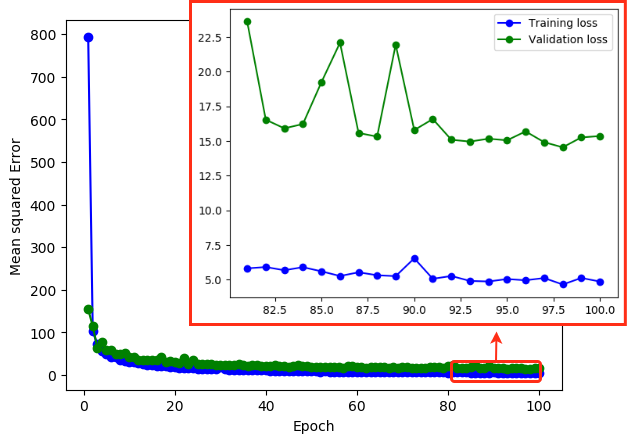
\includegraphics{Images/Experiments/NN/1.initial/exp3_y_5d27075f03f801723c2e360f.png}
  }
  \hfill
  \subfigure[]{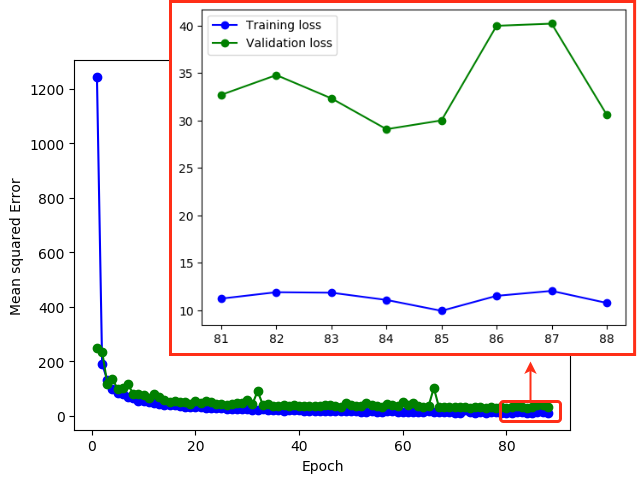
\includegraphics{Images/Experiments/NN/1.initial/exp3_x_5d27075f03f801723c2e360f.png}}
  \caption{Results for site 5d27075f03f801723c2e360f for y estimations (a) and x estimations (b).}
  \label{fig:exp3}
\end{figure}

After using the normalised data instead, the mean of \gls{mse}s dropped significantly, which can be seen on \textbf{\autoref{fig:exp3}}. The \textit{X} model has dropped from a mean of \gls{mse}s from 4967 on the initial model to 10.41 on the training data. The \textit{Y} model has decreased from a mean of \gls{mse}s from 9372 on the initial model to 8.98 on the training data. As can be seen from the graphs, the validation loss is quite high compared to the training loss, which is not an issue of same degree with adjusting the learning rate.

%\begin{figure}[H]
    %\centering
    %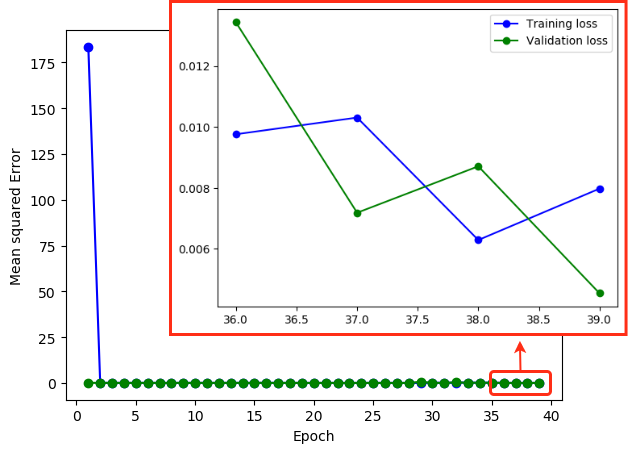
\includegraphics[scale=0.5]{Images/Experiments/NN/1.initial/exp3_floor_5d27075f03f801723c2e360f.png}
    %\caption{Results for site 5d27075f03f801723c2e360f for floor estimations.}
    %\label{fig:exp3_floor}
%\end{figure}
%Here we get a mean on \gls{mse}s for training and validation of 5.6 and 14.9, respectively. The loss is significantly less compared to the previous experiments. 

The most significant change is in the \textit{Floor} model, which decreases the mean of \gls{mse}s to 0.034 for the training dataset and 0.0334 for validation dataset. This proves the assumption about the data making the model unable to properly localise the optimum. Since both reducing the learning rate and using the normalised data combined might lead to even better results. 


\subsection{Result of Fourth Test}
We have also tried a combination of min-max normalised dataset as well as less learning rate, which seems to give good performance. 

\begin{figure}[H]
\centering
  \SetFigLayout{1}{2}
  \subfigure[]{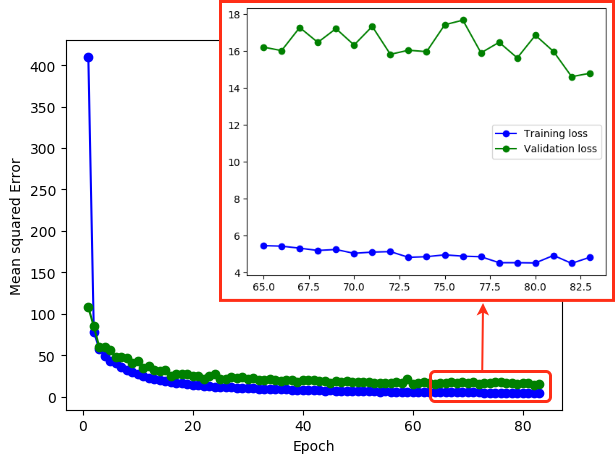
\includegraphics{Images/Experiments/NN/1.initial/exp4_y_5d27075f03f801723c2e360f.png}
  }
  \hfill
  \subfigure[]{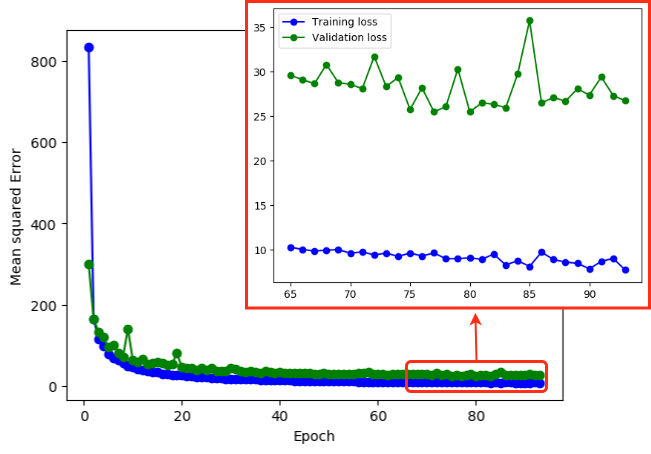
\includegraphics{Images/Experiments/NN/1.initial/exp4_x_5d27075f03f801723c2e360f.png}}
  \caption{Results for site 5d27075f03f801723c2e360f for y estimations (a) and x estimations (b).}
  \label{fig:exp4}
\end{figure}

This for the X and Y model resulted in losses as displayed in \textbf{\autoref{fig:exp3}}, which displays quite a decrease in loss compared to the prior experiments. The graphs seem to perform a bit worse on the validation dataset than for the training dataset, which could be due to slight overfitting.

\begin{figure}[H]
    \centering
    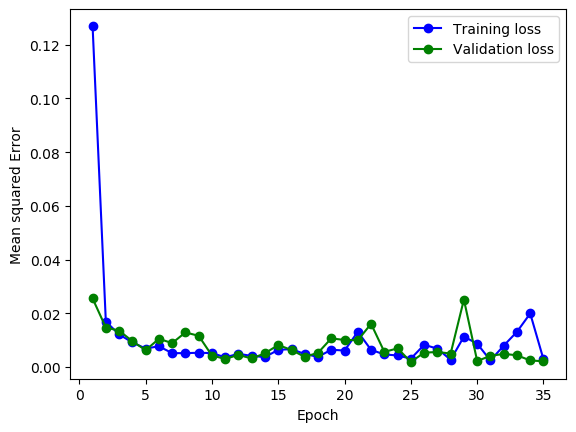
\includegraphics[scale=0.5]{Images/Experiments/NN/1.initial/exp4_floor_5d27075f03f801723c2e360f.png}
    \caption{Results for site 5d27075f03f801723c2e360f for floor estimations.}
    \label{fig:exp4_floor}
\end{figure}

For the \textit{Floor} model, the performance has increased severely since the initial model. The final mean of \gls{mse}s for the training set is 0.0019 and for the validation set is 0.0027.

%We have also calculated the mean of the \gls{mse} for training data and test data is 4.4 and 12.2, respectively. The result, which we achieve for the normalised and less learning rate, seem to perform the best.




\subsubsection{Evaluation of Initial Model}
To evaluate the initial model, we use the \gls{mse}. After determining the most optimal hyper parameters, the k for k-fold should be determined. On \textbf{\autoref{tab:NN_train_initial_results}} and \textbf{\autoref{tab:NN_val_initial_results}}, we see the results for the training data and validation data for the three models (\textit{X}, \textit{Y} and \textit{Floor}). Each model is decribed by the best of k \gls{mse}s, the mean of the \gls{mse}s and the worst of k \gls{mse}s.

\begin{table}[H]
    \centering
    \caption{Results of the training dataset for initial \gls{ann} models, where \textbf{B} stands for the best of k \gls{mse}s, while \textbf{M} stands for the mean of the \gls{mse}s, and \textbf{W} stands for the worst.}
    \begin{adjustbox}{max width=\textwidth}
    \begin{tabular}{m{0.15\textwidth}@{\extracolsep{0.1cm}} m{0.05\textwidth}@{\extracolsep{0pt}} m{0.05\textwidth} m{0.05\textwidth} @{\extracolsep{0.1cm}} m{0.05\textwidth}
    @{\extracolsep{0pt}}
    m{0.05\textwidth} m{0.05\textwidth} @{\extracolsep{0.1cm}} m{0.05\textwidth}@{\extracolsep{0pt}} m{0.05\textwidth} m{0.05\textwidth}}
        \hline
         \multirow{2}{*}{\centering
         \textbf{Description}} & \multicolumn{3}{c}{\textbf{X}} & \multicolumn{3}{c}{\textbf{Y}}& \multicolumn{3}{c}{\textbf{Floor}}\\
         \cline{2-10}
         & \multicolumn{1}{c}{\textbf{B}} & \multicolumn{1}{c}{\textbf{M}}& \multicolumn{1}{c}{\textbf{W}}& \multicolumn{1}{c}{\textbf{B}}& \multicolumn{1}{c}{\textbf{M}}& \multicolumn{1}{c}{\textbf{W}}& \multicolumn{1}{c}{\textbf{B}}& \multicolumn{1}{c}{\textbf{M}}& \multicolumn{1}{c}{\textbf{W}}\\
        \hline\\
        Initial Model & \multicolumn{1}{c}{1073} & \multicolumn{1}{c}{4967} & \multicolumn{1}{c}{$3.1\cdot10^{4}$} & \multicolumn{1}{c}{731} & \multicolumn{1}{c}{9372} & \multicolumn{1}{c}{$7.3\cdot10^{4}$} & \multicolumn{1}{c}{2.67} & \multicolumn{1}{c}{$1.6\cdot10^{5}$} & \multicolumn{1}{c}{$1.6\cdot10^{6}$}
        \\\\
        %\\\hline\\
        Adjusted LR & \multicolumn{1}{c}{72.38} & \multicolumn{1}{c}{669} & \multicolumn{1}{c}{5414} & \multicolumn{1}{c}{77.30} & \multicolumn{1}{c}{1159} & \multicolumn{1}{c}{807} & \multicolumn{1}{c}{1.25} & \multicolumn{1}{c}{8891} & \multicolumn{1}{c}{79966}
        \\\\
        %\\\hline\\
        Normalised Data & \multicolumn{1}{c}{8.03} & \multicolumn{1}{c}{10.41} & \multicolumn{1}{c}{15.89} & \multicolumn{1}{c}{6.75} & \multicolumn{1}{c}{8.98} & \multicolumn{1}{c}{11.63} & \multicolumn{1}{c}{$9.3\cdot 10^{-4}$} & \multicolumn{1}{c}{0.034} & \multicolumn{1}{c}{0.25}
        \\\\
        %\\\hline\\
        Adjusted LR \& Normalised Data & \multicolumn{1}{c}{5.41} & \multicolumn{1}{c}{7.45} & \multicolumn{1}{c}{9.40} & \multicolumn{1}{c}{4.87} & \multicolumn{1}{c}{6.47} & \multicolumn{1}{c}{7.25} & \multicolumn{1}{c}{$9.5\cdot 10^{-4}$} & \multicolumn{1}{c}{0.0019} & \multicolumn{1}{c}{0.0047}
        \\\hline
    \end{tabular}
    \end{adjustbox}
    \label{tab:NN_train_initial_results}
\end{table}

\textbf{\autoref{tab:NN_train_initial_results}} displays the \gls{mse}s for the training dataset. The first row displays information about the initial model before adjusting the learning rate and using the normalised data. Especially, using the normalised data decreases the \gls{mse}s for all the models with both best and worst k \gls{mse}s. Last row describes the model after both adjusting the learning rate and using the normalised data. This model clearly decreases the \gls{mse}s compared to the previous models. The \textit{X} model has decreased from a mean of \gls{mse}s of 4967 to 7.45, and the \textit{Y} model has decreased from a mean of \gls{mse}s of 9372 to 6.47. The model for predicting floors has decreased extremely from a mean of \gls{mse}s of 160000 to 0.0019.

\begin{table}[H]
    \centering
    \caption{Results of the validation dataset for initial \gls{ann} models, where \textbf{B} stands for the best of k \gls{mse}s, while \textbf{M} stands for the mean of the \gls{mse}s, and \textbf{W} stands for the worst.}
    \begin{adjustbox}{max width=\textwidth}
    \begin{tabular}{m{0.15\textwidth}@{\extracolsep{0.1cm}} m{0.05\textwidth}@{\extracolsep{0pt}} m{0.05\textwidth} m{0.05\textwidth} @{\extracolsep{0.1cm}} m{0.05\textwidth}
    @{\extracolsep{0pt}}
    m{0.05\textwidth} m{0.05\textwidth} @{\extracolsep{0.1cm}} m{0.05\textwidth}@{\extracolsep{0pt}} m{0.05\textwidth} m{0.05\textwidth}}
        \hline
         \multirow{2}{*}{\centering
         \textbf{Description}} & \multicolumn{3}{c}{\textbf{X}} & \multicolumn{3}{c}{\textbf{Y}}& \multicolumn{3}{c}{\textbf{Floor}}\\
         \cline{2-10}
         & \multicolumn{1}{c}{\textbf{B}} & \multicolumn{1}{c}{\textbf{M}}& \multicolumn{1}{c}{\textbf{W}}& \multicolumn{1}{c}{\textbf{B}}& \multicolumn{1}{c}{\textbf{M}}& \multicolumn{1}{c}{\textbf{W}}& \multicolumn{1}{c}{\textbf{B}}& \multicolumn{1}{c}{\textbf{M}}& \multicolumn{1}{c}{\textbf{W}}\\
        \hline\\
        Initial Model & \multicolumn{1}{c}{780.27} & \multicolumn{1}{c}{3077.49} & \multicolumn{1}{c}{13291.79} & \multicolumn{1}{c}{681.45} & \multicolumn{1}{c}{2407.32} & \multicolumn{1}{c}{7130.71} & \multicolumn{1}{c}{2.02} & \multicolumn{1}{c}{8538.34} & \multicolumn{1}{c}{$85035.24$}
        \\\\
        %\\\hline\\
        Adjusted LR & \multicolumn{1}{c}{62.50} & \multicolumn{1}{c}{2298.73} & \multicolumn{1}{c}{5413.96} & \multicolumn{1}{c}{57.66} & \multicolumn{1}{c}{230.59} & \multicolumn{1}{c}{966.00} & \multicolumn{1}{c}{0.81} & \multicolumn{1}{c}{533.03} & \multicolumn{1}{c}{5300.95}
        \\\\
        %\\\hline\\
        Normalised Data & \multicolumn{1}{c}{14.57} & \multicolumn{1}{c}{21.21} & \multicolumn{1}{c}{39.74} & \multicolumn{1}{c}{12.31} & \multicolumn{1}{c}{19.74} & \multicolumn{1}{c}{41.58} & \multicolumn{1}{c}{0.00094} & \multicolumn{1}{c}{0.0334} & \multicolumn{1}{c}{0.25}
        \\\\
        %\\\hline\\
        Adjusted LR \& Normalised Data & \multicolumn{1}{c}{12.26} & \multicolumn{1}{c}{17.29} & \multicolumn{1}{c}{26.54} & \multicolumn{1}{c}{10.90} & \multicolumn{1}{c}{14.41} & \multicolumn{1}{c}{19.13} & \multicolumn{1}{c}{0.00041} & \multicolumn{1}{c}{0.0027} & \multicolumn{1}{c}{0.014}
        \\\hline
    \end{tabular}
    \end{adjustbox}
    \label{tab:NN_val_initial_results}
\end{table}

\textbf{\autoref{tab:NN_val_initial_results}} displays the \gls{mse}s for the validation dataset. The different \gls{mse}s follow similar values to the \gls{mse}s training data in \textbf{\autoref{tab:NN_train_initial_results}}. Similarly, adjusting the learning rate and using the normalised data has decreased the models for \textit{X}, \textit{Y} and \textit{Floor} respectively to 17.29, 14.41 and 0.0027. The mean of the \gls{mse}s for the Floor model is quite similar from training and validation. Where the models for \textit{X} and \textit{Y} increases the mean of \gls{mse}s by 9.84 and 7.94 respectively for validation. This increase could potentially mean that the model is slightly overfitting, since it performs worse on the validation data.

In general, for all of the initial \gls{ann} experiments, none of them have a high degree of overfitting. Meaning that the model does not over specialise for the training data and thereby get good results for the training data while getting bad results for the validation data. This might be an indication of the initial model might not have enough expressive power. So for the next model, we will try to increase the expressive power of the model.

\subsection{Second Model}
We have also experimented with a deeper model. 
\begin{table}[H]
    \centering
    \caption{Model Specification for a deeper \gls{ann} experiment.}
    \begin{tabular}{m{0.3\textwidth}m{0.2\textwidth} m{0.2\textwidth}}
        \hline
        \multicolumn{1}{c}{\textbf{Description}} & \multicolumn{1}{c}{\textbf{Neurons}} & \multicolumn{1}{c}{\textbf{Activation}}\\
        \hline
        
        Input Layer         &   \multicolumn{1}{c}{$N$} & \multicolumn{1}{c}{None}        \\
        1. Hidden Layer     &   \multicolumn{1}{c}{$N$}  & \multicolumn{1}{c}{ReLU}     \\
        2. Hidden Layer     &   \multicolumn{1}{c}{$\frac{1}{2}N$}  & \multicolumn{1}{c}{ReLU}     \\
        3. Hidden Layer         &   \multicolumn{1}{c}{$\frac{1}{2}N$} & \multicolumn{1}{c}{ReLU}        \\
        4. Hidden Layer         &   \multicolumn{1}{c}{$\frac{1}{2}N$} & \multicolumn{1}{c}{ReLU}        \\
        5. Hidden Layer         &   \multicolumn{1}{c}{$\frac{1}{4}N$} & \multicolumn{1}{c}{ReLU}        \\
        Output Layer     &   \multicolumn{1}{c}{$1$}  & \multicolumn{1}{c}{None}     \\
        \hline
    \end{tabular}
    \label{tab:NN02}
\end{table}
We have trained this model using the normalised dataset. For X estimations, we achieves mean of \gls{mse}s of 124.72 and 18.65 for training and validation dataset. The best of k mean of \gls{mse}s for X estimations are 5.89 and 10.85 for training and validation, while the worst of k mean of \gls{mse}s are 532.67 and 31.76.

For Y estimations, we achieve a mean of \gls{mse}s of 13.08 and 115.10 for training and validation, respectively. For the best k mean of \gls{mse}s, we get 5.94 \& 11.08 for training and validation, respectively, while we get 33.61 and 520.30 of the worst k.

For the floor estimations, we achieve a mean of \gls{mse}s of 5.54 and 0.99 for the training and validation. For the best k mean of \gls{mse}s, we get 0.23 and 0.21, while we get for the worst 3.27 and 2.39 for training and validation.

So looking at the results overall, it does not seem to be an improvement compared to the initial models. Perhaps with further testing of increasingly deep model, we might get a good performance, but due to time constraints we cannot keep testing models.


\subsection{Reflection on Experiments}
\todo{Abi ved hvad der menes, så han fixer :) -flet ind således at det står imellem intial model og second model}
%In general, for all of the \gls{ann} experiments, none of them have a high degree of overfitting. Meaning that the model does not over specialise for the training data and thereby get good results for the training data while getting bad results for the validation data. This might be an indication of the initial model might not have enough expressive power. So for the next model, we will try to increase the expressive power of the model. 
The training time with 10-fold cross validation is long, so we would like to test with 5-fold cross validation. If we do not identify a big difference in performance, we will be using 5-fold cross validation. 
%The mean of \gls{mse}s for training and validation data for 5-fold cross validation is 4.6 and 13.3, respectively. As this difference is minor compared to the 10-fold cross validation, we will be using 5-fold henceforth in order to save training time.